\cotefile{89}
\scanpage{12}
Ceci étant, on \unsure{a} des équivalences de catégories

\diagram{\begin{tikzcd}[ampersand replacement=\&,column sep=small,row sep=large]
\& \bigl(\underline{\mathrm{Tors}}(V)\bigr)
  \arrow[dl,leftrightarrow,"\approx"'] \arrow[dr,leftrightarrow,"\approx"] \& \\
{\llap{\text{(7)}\qquad}\displaystyle\prod_{i\in\tau}\bigl(\mathrm{Tors}(D_i)\bigr)}
 \& \& {\displaystyle\prod_{i\in\tau'}\bigl(\mathrm{Tors}(D_i)\bigr).}
\end{tikzcd}}

Notons que pour une droite vectorielle $D$ sur $\mathbb F_3$, la catégorie $\mathrm{Tors}(D)$ est isomorphe canoniquement \unsure{à|:} celle des ens. $E$ de cardinal $3$, munis d'une bijection
\[
\underset{\substack{\text{(ens des 2}\\\text{orientations de }E,\\
\text{i.e. des deux}\\\text{permutations circulaires}\\
\text{de }E\text{ inverses}\\\text{l'une de l'autre}}}{\omega_E}
 \simeq D^{*}
\]
de sorte que la catégorie $\prod_{i\in\tau}\bigl(\mathrm{Tors}(D_i)\bigr)$ peut être regardée comme celle des familles à deux éléments, indexées par $\tau$, d'ensembles de cardinal $3$
\[
(\deleted{F}P_i)_{i\in\tau}
\]
munis chacun d'une bijection
\[
\omega_{P_i}\simeq D_i^{*}\qquad(i\in\tau)
\]
-- et de même pour la catégorie $\prod_{i\in\tau'}\bigl(\mathrm{Tors}(D_i)\bigr)$.
% archive sheet number: 11
\scanpage{13}
On peut aussi l'interpréter, \inserted{via $(P_i)_{\unsure{i\in\tau|i'\in\tau|i\in T}}\longmapsto\coprod_{i\in\tau}P_i$,} comme la catégorie des ensembles $E$ de cardinal $6$, munis d'une partition \inserted{$(P_i)_{i\in\tau}$} de type $(3,3)$ indexée par $\tau$, et pour chaque $i\in\tau$ d'une bijection $\omega_{P_i}\simeq D_i^*$. Ainsi les deux équivalences (7) fournissent une équivalence

\diagram{\begin{tikzcd}[ampersand replacement=\&,column sep=large]
{\llap{\text{(8)}\quad}\begin{array}[t]{@{}l@{}}
 \text{Catégorie des ens. }E\text{ de}\\
 \text{cardinal }6,\text{ munis d'une}\\
 \text{partition }\inserted{(P_i)_{i\in\tau}}\text{ de type }(3,3),\\
 \text{indexée par }\tau,\text{ et d'une}\\
 \text{\deleted{\unsure{f|famille} paire} de bijections}\\
 D_i^*\simeq\omega_{P_i}
\end{array}} \arrow[r,"\approx"] \&
{\begin{array}[t]{@{}l@{}}
 \text{Catégorie analogue}\\
 \text{définie en termes}\\
 \text{de }\tau'\text{ et de}\\
 (D_i^*)_{i\in\tau'}
\end{array}}
\end{tikzcd}}

Quand \inserted{(\unsure{gardant|grâce à} $V$)} on échange les rôles de $\tau$ et de $\tau'$, il est évident que le diagramme d'équivalences (7) reste le même à symétrie près, et que l'équivalence (8) est donc remplacée par \deleted{\unsure{l'}}\inserted{une} équivalence, \inserted{canoniquement} quasi-inverse de la précédente.

Les catégories source et but dans (8) sont définies en termes de la famille, \deleted{\unsure{de}}indexée par $P(V)=\tau\amalg\tau'$, d'ensembles à deux éléments $\omega_i=D_i^*\deleted{\unsure{\omega}}$ (dont la donnée équivaut à celle de la famille des droites \deleted{\unsure{D}}\unsure{Vect.|vect.} $D_i$ sur $\mathbb F_3$),
% archive sheet number: 12
\scanpage{14}
vu que $\deleted{\mathbb F_3}$ l'on \unsure{a}
\[
\mathbb F_3^*=\{\pm1\}\qquad\big).
\]

\deleted{Ainsi} \inserted{Notons que} la donnée de $\deleted{\{}(\omega_i)_{i\in\tau}\deleted{\}}$ permet ainsi de réconstituer \inserted{(à isom. can. près)} la famille $(D_i)_{i\in\tau}$ de droites \inserted{vectorielles sur $\mathbb F_3$} (via $D_i=\omega_i\amalg\{0\}\ \ldots$), donc le vectoriel $V=\prod_{i\in\tau}D_i$ sur $\mathbb F_3$, donc aussi \inserted{le plan vectoriel} $V=\prod_{i\in\tau}D_i$ avec la paire de droites indexée par $\tau$, d'où la paire complémentaire $(D_i)_{i\in\tau'}$. La \deleted{\unsure{On a|trouve|Donc} ainsi en fait} donnée d'une famille $(\omega_i)_{\unsure{v|i}\in\tau}$ d'ens à deux éléments, indexée par $\tau$, équivaut à celle d'un \uline{carré} \inserted{comb.} $Q$, admettant $\tau$ comme ens des diagonales. On trouve \inserted{\unsure{ainsi}} \deleted{\unsure{donc|d'une|une}} équivalence

\diagram{\begin{tikzcd}[ampersand replacement=\&,column sep=large]
{\llap{\text{(9)}\quad}\begin{array}[t]{@{}l@{}}
\text{Carrés combinatoires}\\Q
\end{array}} \arrow[r,leftrightarrow,"\approx"] \&
{\begin{array}[t]{@{}l@{}}
\text{plans vectoriels }\inserted{V}\text{ sur }\mathbb F_3,\\
\text{munis d'une paire}\\
\text{de droites vectorielles}\\
(D_{\unsure{v|i}})_{i\in\tau}
\end{array}}
\end{tikzcd}}

dans cette équivalence, donc, \deleted{$\tau$ correspond à} \inserted{on a}

\deleted{\unsure{diag|Diag $Q$}}
\[
\left\{\begin{aligned}
\tau&\simeq\mathrm{diag}_{Q} &&\text{et}\quad D_i^*\simeq d_i\quad\text{pour }i\in\tau\\
S_Q&=\bigcup_{i\in\tau}D_i^*=\coprod_{i\in\tau}D_i^*\\
\inserted{A_Q}&\inserted{=\prod_{i\in\tau}D_i^*\simeq V^*-\bigcup_{\unsure{i\in\tau|i\in T}}D_i^*}\;
 \tikz[baseline=-.25ex]{\draw (0,0)--(.10,.16)--(.22,.42) (.10,.16)--(.21,0);}
\end{aligned}\right.
\tag*{(10)}
\]
\margin{$\tikz[baseline=-.25ex]{\draw (0,0)--(.10,.16)--(.22,.42) (.10,.16)--(.21,0);}
=\bigcup_{i\in\tau'} D_i^*$}
où $d_i$ est l'ensemble des deux sommets de $Q$ qui constituent la diagonale $i$
% archive sheet number: 13
\scanpage{15}
\deleted{\unsure{On|Le|Rien}} On a d'ailleurs
\[
\underset{\substack{\text{ens d'arêtes}\\\text{de }Q}}{A_Q}
 \simeq\underset{\substack{\text{produit}\\\text{des deux}\\\text{diagonales de }Q}}{\prod_{i\in\tau}D_i^*}
 \simeq V^*-\bigcup_{i\in\tau}D_i^*
 =\bigcup_{i\in\tau'}D_i^*=
\]
ce qui montre que \deleted{\unsure{$V^*$|$V$} \unsure{ou}} le carré défini par \deleted{\unsure{l'ens|l'ens.}}\inserted{la paire} \deleted{\unsure{des}} $(D_i)_{i\in\tau'}$ de \deleted{droites} de $V^*$ complémentaire de la paire $(D_i)_{i\in\tau}$ \unsure{d'identifie|s'identifie} au carré dual $DQ$ de $Q$. Si on désigne par $V(Q)$ le \inserted{plan} vectoriel sur $\mathbb F_3$ défini par $Q$, on trouve donc un isomorphisme
\[
V(DQ)\xrightarrow{\overset{\alpha_Q}{\sim}}V(Q)
\tag*{(11)}
\]
et de façon symétrique on a
\[
V\bigl(\underset{\substack{\rotatebox{90}{$\simeq$}\\DDQ}}{\deleted{\unsure{D}}Q}\bigr)
 \xrightarrow{\alpha_{DQ}}V(DQ)
\tag*{(\unsure{12|11})}
\]
Ceci posé, on a la relation
\[
\alpha_{\deleted{\unsure{D}}Q}\,\alpha_{DQ}=-\mathrm{id}_{V(Q)}
=V\bigl(\underset{\substack{\text{antipodisme}\\\text{de }Q}}{\underbrace{\underline{a}_{Q}}}\bigr)
\tag*{(\unsure{12|13})}
\]
et de $=$ bien entendu
\[
\alpha_{DQ}\,\alpha_Q=-\mathrm{id}_{V(DQ)}=V(\underline{a}_{DQ}).
\]
% archive sheet number: 14
\scanpage{16}
Soient $V$ un Module \deleted{loc.} libre \inserted{de rang $2$} sur un \deleted{topos loc. annelé}\inserted{anneau $\Lambda$}, d'où $P(V)=$ ens des ``droites vectorielles'' dans $V$ (i.e des sous modules \inserted{\deleted{\unsure{loc.}}} \deleted{libres \unsure{d|de}} inversibles facteurs directs),

\deleted{et $P(V)^{\unsure{'|!}}=$}

\[
\begin{aligned}
V^*&=\text{ens. des éléments de }V\text{ partout }\ne0\quad(\Longleftrightarrow\text{ qui}\\
&\hspace{2em}\text{font partie d'une base})
\end{aligned}
\tag*{(1)}
\]
\[
\begin{aligned}
P(V)^!&=V^*/\Lambda^*\hookrightarrow P(V)\quad\text{l'ens des ``droites dans }V\text{''}\\
&\text{qui sont des modules libres de rang }1.
\end{aligned}
\tag*{(2)}
\]
On a envie d'expliciter comment on récupère \inserted{le $\Lambda$-module} $V$ à l'aide de l'ens $P(V)^!$, muni d'une structure supplémentaire, qui est \deleted{un} essentiellement le $\Lambda^*$-\deleted{\unsure{fibré}}\unsure{torseur} relatif (ensembliste) $V^*$ sur $P(V)^!=X$. Pour $x\in P(V)^!$, soit $D_x\subset V$ la droite vectorielle correspondante, et posons
\[
T_x=D_{\unsure{a|x}}^*\quad(\deleted{\unsure{A}}\Lambda^*\text{-torseur})
\tag*{(3)}
\]
Soit de plus
\[
\omega_V=\det(V)^*\qquad(\text{un }\Lambda^{\unsure{*|\alpha|\circ}}\text{-torseur}
\tag*{(4)}
\]
Sur $P(V)^!$ on a la relation binaire de disjonction
\[
x,y\in P(V)^!\quad\text{``\uline{disjoints}''}\quad\text{\unsure{ass|ssi}}\quad V\simeq D_x\oplus D_y
\]
(si $\Lambda$ est un corps, cela équivaut à $x\ne y$; si $\Lambda$ est local, cela équivaut à $x_0\ne y_0$ (l'indice $0$
% archive sheet number: 15
\scanpage{17}
désignant la réduction mod. idéal maximal).

Si $x$ et $y$ sont disjoints, alors \inserted{(et alors seulement)} \deleted{\unsure{l'applicat|l'applicati|l'appl.}}
\[
\begin{aligned}
 (u,v)&\unsure{\mathrel{\vdash\mkern-8mu\dashv}|\mapsto}u\wedge v\\
 D_x\times\unsure{D|D_x|D_y}&\longrightarrow\det V
\end{aligned}
\]
induit
\[
T_x\times T_y\longrightarrow\omega_V
\]
qui se factorise par un \inserted{iso}morphisme
\[
\underbrace{T_x\wedge T_y}_{\substack{\text{produit contracté}\\\text{de }\Lambda^{\unsure{*|\alpha}}\text{-torseurs}}}\simeq\omega_V
\tag*{(5)}
\]
\deleted{\unsure{appelé|noté}} l'image \inserted{dans $\omega_V$} de $(u\wedge v)$ par cette application sera encore noté $u\wedge v$. On aura
\[
u\wedge v=-v\wedge u
\tag*{(6)}
\]
\margin{NB $-1\in\Lambda^*$, d'où \unsure{pour|pose}, pour un $\Lambda^*$-torseur $T$, et $u\in T$, $-u\overset{\mathrm{def}}{=}(-1).u$ )}

Soient $x,y$ \inserted{$\in P(V)^!$} disjoints, et $z\in P(V)^!$ quelc, soient
\[
u\in T_{\unsure{a|x}},\ v\in T_y,\ w\in T_z
\]
considérons la relation
\[
u\wedge v=v\wedge w=w\wedge u
\tag*{(7)}
\]
équivalente à
\[
\deleted{\unsure{u|v}}w\wedge v=v\wedge u=u\wedge w\qquad,
\tag*{(7$'$)}
\]
on vérifie de suite qu'elle équivaut à
\[
u+v+w=0
\tag*{(8)}
\]
et qu'elle implique que $z$ est disjoint de $x,y$.
% archive sheet number: 16
\scanpage{18}
Je dis que \inserted{le $\Lambda$-module} $V$ se réconstitue \inserted{(au moins si $\Lambda$ est un corps)} à partir de

a) l'ens $P:=P(V)^!$.

b) la famille des \inserted{$\Lambda$-torseurs} $(T_x)_{x\in P\deleted{(V)^!}}$ -- i.e. le \inserted{$\Lambda^*\deleted{\unsure{P(V)^!|P}}$-}torseur relatif $\coprod_{x\in P(V)^!} T_x=V^*$ sur $P\deleted{(V)}$
% slanted
\margin{équivaut à la donnée de l'ens $V^*$, avec l'opération (libre) de $\Lambda^*$ sur $V^*$ $\big\{$}

c) le $\Lambda^*$-torseur $\omega=\omega_V$

d) la donnée de la relation de disjonction dans $P\deleted{(V)^!}\inserted{=P(V)^!}$ [ou ce qui revient au $=$, dans $V^*$ -- cette relation étant \inserted{bi-}stable par l'opération $\Lambda^*$ (i.e. $u,v$ disjoints $\Rightarrow\lambda u,\mu v$ disjoints pour $\lambda,\mu\in\Lambda^*$)].
% slanted
\margin{Si $\Lambda$ est un corps, cette relation est la relation triviale $x\ne y$, et ne demande pas de donnée suppl. $\big[$}

\deleted{\unsure{d)|e)} le $\Lambda^*$-torseur $\omega_{\unsure{V}}=\omega_V$}

\unsure{e)|f)} la donnée, pour $x,y$ disjoints, de l'isom de $\Lambda^*$-torseurs
\[
T_x\wedge T_y\simeq\omega\qquad\text{noté}\quad
u\mathbin{\underset{\Lambda_{\unsure{*}}}{\wedge}}v\mapsto u\wedge v
\]

En effet, pour \deleted{\unsure{$x,y,z\in$}} $u,v,w$ dans $V^*$, deux à deux disjoints, on trouve
\[
u+v+w\quad\Longleftrightarrow\quad u\wedge v=v\wedge w=w\wedge u
\]
donc on arrive à trouver la loi de composition \inserted{partielle} $(u\unsure{,|+}v)\mapsto u+v$ sur $V^*$ pour $u,v$ \uline{disjoints}.

\deleted{On \unsure{en|a}} Dans le cas où $\Lambda$ est un corps, posant
\[
\left\{\begin{aligned}
V&=V^*\amalg\{0\}\\
D_x&=T_x\cup\{0\}\subset V
\end{aligned}\right.
\]
les $D_x$ sont des droites vectorielles sur $\Lambda$, et on
% archive sheet number: 17
\scanpage{19}
définit $u+v$ $(u,v\in V^*)$ séparément quand $u$ ou $v=0$ (comme étant $v$ resp. $u$), quand $u,v\in V^*$ et $u,v$ dans un $=$ $D_x$ (par la loi additive de $D_x$), et quand $u+v$ sont disjoints par \deleted{la \unsure{pr|p}} comme $-w$, où $w$ est l'\uline{unique} $w\in V^*$ qui soit disj. de $u,v$ et tel que $u\wedge v=v\wedge w=w\wedge u$. Pour pouvoir réaliser cette construction, on a besoin des \deleted{ceci} propriétés que voici sur les données a) b) c) [d)] e) :

a) Pour $x,y,z$ \inserted{$\in P$} mutuellement disjoints, on peut trouver $u\in T_x$, $v\in T_y$, $w\in T_z$ tels que l'on ait
\[
u\wedge v=v\wedge w=w\wedge u\qquad(\text{soit }\alpha\mathrel{\unsure{+|\in}}\omega)
\]
(et alors on peut $=$ supposer que $u$ \inserted{ou} $v$ \inserted{ou} $w$ \deleted{\unsure{ou $\alpha$|ou $x$}} soit donné d'avance).
% archive sheet number: 18
\scanpage{20}
$\mathrm{Pol}\ \mathrm{top}\longrightarrow\mathrm{Pol}\ \mathrm{comb}$ ess.$^{\mathrm t}$ surjectif : \unsure{dém. abstraite|dim. abstraite}

\uline{Foncteur réalisation topologique}

dualité : échange de $S$ et $A$

\figure{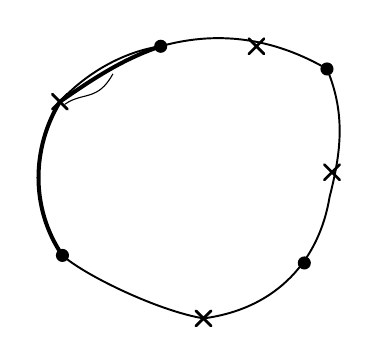
\begin{tikzpicture}[x=0.032cm,y=-0.032cm,line cap=round,line join=round]
\draw[line width=.7pt] (12,30) .. controls (23,18) and (38,10) .. (52,8)
 .. controls (77,1) and (99,6) .. (118,17)
 .. controls (126,36) and (123,52) .. (119,68)
 .. controls (115,92) and (99,112) .. (69,116)
 .. controls (51,113) and (22,99) .. (13,91)
 .. controls (1,73) and (0,50) .. (12,30);
\draw[line width=1.45pt] (13,91) .. controls (0,72) and (1,48) .. (12,30)
 .. controls (25,21) and (37,13) .. (52,8);
\draw (14,31) .. controls (21,26) and (27,30) .. (33,19);
\foreach \x/\y in {52/8,118/17,109/94,13/91}{\fill (\x,\y) circle[radius=2.6];}
\foreach \x/\y in {12/30,90/8,120/58,69/116}{
\draw[line width=1pt] (\x-3,\y-3)--(\x+3,\y+3) (\x-3,\y+3)--(\x+3,\y-3);}
\end{tikzpicture}}

point de vue ens. ordonnés \quad $P=S\amalg A$

\deleted{\unsure{dont}} ($S$ él. minimaux, $A$ éléments maximaux

chaque élément minimal \unsure{majorant|majoré}

chaque élément minimal majoré \inserted{\unsure{str.$^{\mathrm t}$|strt|strict.}} par \unsure{exactemt|exactement} deux él. \unsure{dist.|div.|distincts} maximaux)

chaque élément maximal minoré par exactement deux éléments \unsure{combi.|comb.} minimaux)

ici dualité : renversement de la relation d'ordre

Composantes connexes \deleted{\unsure{des}} \unsure{sont|v$^{\mathrm t}$|v.t.} des \unsure{cercles|ens|ens.} comb.

\deleted{point de vue} polygone combin. (trois définitions comb. équiv.)

Point de vue \uline{ens. de base $S$} (valable si les comp. connexes sont \uline{d'ordre $\geq3$})

$A\hookrightarrow\unsure{\mathfrak P|\mathcal P|P}_2(S)$ structure ens. de parties à deux éléments de $S$ (appelées \uline{arêtes}) tel que $\forall\ s\in S$ appartient à exactemt deux arêtes

Point de vue dual : structure sur $A$, d'un ens $S\hookrightarrow\mathfrak P_2(A)$ (qu'on appellera les ``sommets'')

Point de vue ordres circulaires (cas des polygônes d'ordre $\geq3$) : donnée sur $S$ (ou $A$) d'une paire d'ordres circulaires \inserted{(i.e. permutations transitives)} inverses l'un de l'autre -- une \uline{orientation} de $\deleted{\unsure{P}}$ $\Pi$ correspond au choix de l'un des deux ordres circulaires en question.
% archive sheet number: 19
\scanpage{21}
Orientation d'une \uline{arête} : par choix d'une ``origine''.
% slanted
\margin{Orientations opposées}
Orientation induite sur le bord de l'arête (extrémité -- origine)

Orientation d'un contour combinatoire : choix d'une orientation sur chaque arête, de telle façon que pour tt sommet $s$, les deux orientations induites sur $s$ soient opposées
\diagram{\begin{tikzcd}[ampersand replacement=\&,row sep=.2em,column sep=2em]
{} \arrow[dr] \& \& {}\\
\& \bullet \arrow[ur] \&
\end{tikzcd}}

\deleted{\unsure{Rem}} Relations avec le cas topologique ; orientation d'un segment topologique, d'une $1$-variété topologique

\uline{Théorème} a) Tout \uline{\unsure{polygône|polygone}} combinatoire admet \unsure{exactemt|exactement} $2$ orientations, \unsure{opposées} \deleted{\unsure{l'une à l'autre}} l'une de l'autre.
% slanted
\margin{S'il y a $r$ comp. connexes, alors il y a $2^r$ orientations}

b) À toute orientation $\omega$ \inserted{d'un contour,} correspond un unique \unsure{autom|bijection} $\rho_\omega$ tel que

1) $\rho_\omega$ conserve l'orientation

2) $\forall s\in S$, $\deleted{\unsure{\rho}}(s,\rho_\omega(s))$ soit une \uline{arête} $\underline a$, dont l'origine $o_\omega(a)$ soit $s$.
% slanted
\margin{\unsure{$\alpha$)|2)|b)} $\forall s\in S$, $\deleted{\unsure{\rho}}\rho(s)$ est adjacent à $s$\\
\unsure{$\beta$)|3)} $\forall a\in A$, $\rho(a)$ est adj. à $a$ \quad NB\\
$\alpha$) et $\beta$) sont \unsure{équivalents|équivalentes}, s'il n'y a pas de comp. bigone}

\deleted{c) $\omega\mapsto\rho_\omega$ est une \unsure{corr.|corresp.} $1$-$1$ entre l'ens des or. et l'ens des \unsure{auto.|autom.} de $\Pi$ tels que \illegible{1}}

\uline{NB} 2) caractérise déjà $\rho_\omega$, si les comp. de $\Pi$ sont d'ordre $\geq3$.

\deleted{\unsure{c)}} c) $\omega\mapsto\rho_\omega$ induit une bij. entre l'ens des orientations de $\Pi$, et l'ens des \unsure{autom|automorphismes} de $\Pi$ qui satisfont :

\uline{NB} La description des orientations via $\rho$ est autoduale. Orienter $\Pi$ en un sommet $s$ revient à choisir

\figure{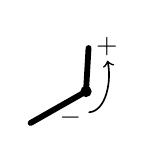
\begin{tikzpicture}[x=.8cm,y=.8cm,line cap=round,line join=round]
\draw[line width=2.1pt] (-.88,-.50)--(0,0)--(.04,.69);
\fill (0,0) circle[radius=.09];
\draw[->,line width=.6pt] (.05,-.33) .. controls (.32,-.31) and (.41,.17) .. (.34,.49);
\node at (.33,.72) {$+$}; \node at (-.25,-.41) {$-$};
\end{tikzpicture}}
l'arête ``origine'' et l'arête extrémité autour de $s$
% archive sheet number: 20
